\documentclass[8pt,executivepaper]{article}
\usepackage[utf8]{inputenc}
\usepackage[spanish]{babel}
\usepackage{amsmath}
\usepackage{amsfonts}
\usepackage{amssymb}
\usepackage{graphics}
\usepackage{graphicx}
\usepackage[left=1cm,right=1cm,top=2cm,bottom=2cm]{geometry}
\usepackage{imakeidx}
\makeindex[columns=3, title=Alphabetical Index, intoc]
\usepackage{listings}
\usepackage{xcolor}
\usepackage{multicol}
\usepackage{changepage}
\usepackage{float}
\usepackage{cite}
\usepackage{url}
\usepackage{hyperref}
\usepackage{pdfpages}

\definecolor{codegreen}{rgb}{0,0.6,0}
\definecolor{codegray}{rgb}{0.5,0.5,0.5}
\definecolor{codepurple}{rgb}{0.58,0,0.82}
\definecolor{backcolour}{rgb}{0.95,0.95,0.92}

\lstdefinestyle{mystyle}{
    backgroundcolor=\color{backcolour},
    commentstyle=\color{codegreen},
    keywordstyle=\color{magenta},
    numberstyle=\tiny\color{codegray},
    stringstyle=\color{codepurple},
    basicstyle=\ttfamily\footnotesize,
    breakatwhitespace=false,
    breaklines=true,
    captionpos=b,
    keepspaces=true,
    numbers=left,
    numbersep=5pt,
    showspaces=false,
    showstringspaces=false,
    showtabs=false,
    tabsize=3
}

\lstset{style=mystyle}
\author{González Pardo Adrian}
\date{Marzo 2020}

\title{Reporte de practica 6}
\newcommand\tab[1][1cm]{\hspace*{#1}}
\begin{document}
\maketitle
\section{Código VHDL}
\subsection{Mux de 16 canales}
\lstinputlisting[language=VHDL]{sourcesCodes/muxGral.vhd}
\subsection{Mux de 2 canales}
\lstinputlisting[language=VHDL]{sourcesCodes/mux2.vhd}
\subsection{Demux de 16 canales}
\lstinputlisting[language=VHDL]{sourcesCodes/demuxG.vhd}
\subsection{Registro de 16 bits}
\lstinputlisting[language=VHDL]{sourcesCodes/registro.vhd}
\subsection{Barrel-Shifter}
\lstinputlisting[language=VHDL]{sourcesCodes/barrel.vhd}
\subsection{Archivo de registros}
\lstinputlisting[language=VHDL]{sourcesCodes/archRegistros.vhd}
\section{Test-Bench VHDL Código}
\subsection{Test-Bench registro}
\lstinputlisting[language=VHDL]{testBenchCodes/registroTB.vhd}
\subsection{Test-Bench barrel shifter}
\lstinputlisting[language=VHDL]{testBenchCodes/barrelTB.vhd}
\subsection{Test-Bench archivo de registros}
\lstinputlisting[language=VHDL]{testBenchCodes/archRegTB.vhd}
\subsubsection{Archivos de entrada y salida para esta sección}
\textbf{Archivo de entrada (input.txt)}
\lstinputlisting{txts/input.txt}
\clearpage
\textbf{Archivo de salida (output.txt)}
\lstinputlisting{txts/output.txt}
\subsubsection{Tabla de resultados de la salida}
\begin{tabular}{|c|c|c|c|c|c|c|c|c|c|}
  \hline
  RR1 & RR2 & SHAMT & WREG & WD & WR & SHE & DIR & RD1 & RD2\\
  \hline
  8 & 4 & 0000 & 5 & 0F86 & 1 & 0 & 1 & 0000 & 0000 \\
  1 & 0 & 0000 & 1 & 0089 & 1 & 0 & 0 & 0089 & 0000 \\
  2 & 1 & 0000 & 2 & 0072 & 1 & 0 & 0 & 0072 & 0089 \\
  3 & 0 & 0000 & 3 & 0123 & 1 & 0 & 0 & 0123 & 0000 \\
  4 & 0 & 0000 & 4 & 0053 & 1 & 0 & 0 & 0053 & 0000 \\
  1 & 2 & 0000 & F & FFFF & 0 & 0 & 0 & 0089 & 0072 \\
  3 & 4 & 0000 & E & EEEE & 0 & 0 & 0 & 0123 & 0053 \\
  1 & 2 & 0011 & 2 & 1234 & 1 & 1 & 0 & 0089 & 0448 \\
  3 & 0 & 0101 & 4 & 5555 & 1 & 1 & 1 & 0123 & 0000 \\
  1 & 2 & 0000 & F & FFFF & 0 & 0 & 0 & 0089 & 0448 \\
  3 & 4 & 0000 & E & EEEE & 0 & 0 & 0 & 0123 & 0009 \\
  8 & 4 & 0000 & 5 & 0F86 & 1 & 0 & 1 & 0000 & 0000 \\
  \hline
\end{tabular}
\section{Simulaciones}
\subsection{Registro}
\begin{center}
  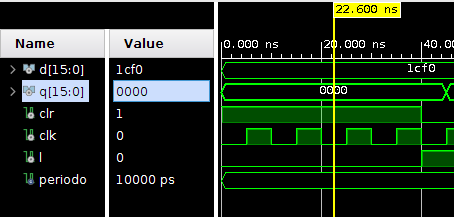
\includegraphics[scale=0.5]{imgs/uno.png}\\
  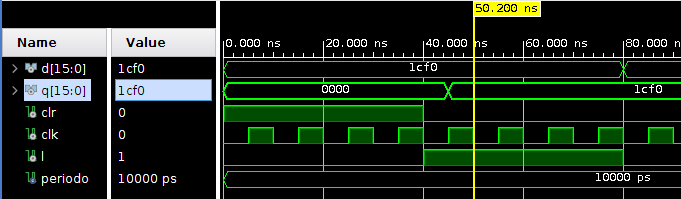
\includegraphics[scale=0.5]{imgs/dos.png}\\
  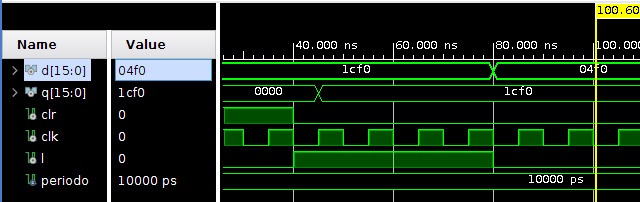
\includegraphics[scale=0.5]{imgs/tres.png}\\
  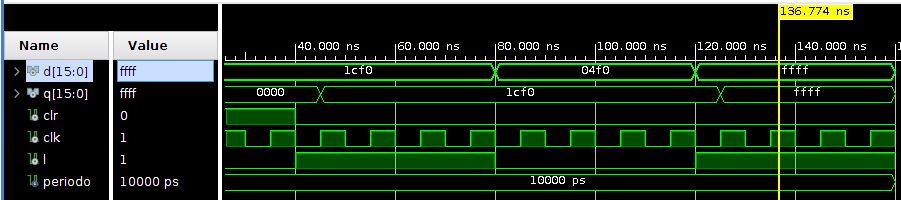
\includegraphics[scale=0.5]{imgs/cuatro.png}\\
\end{center}
\subsection{Barrel-Shifter}
\begin{center}
  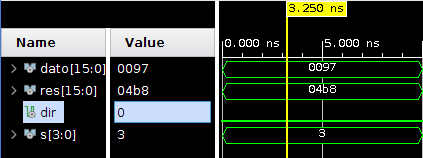
\includegraphics[scale=0.5]{imgs/unoBarrel.png}\\
  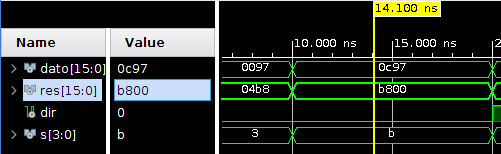
\includegraphics[scale=0.5]{imgs/dosBarrel.png}\\
  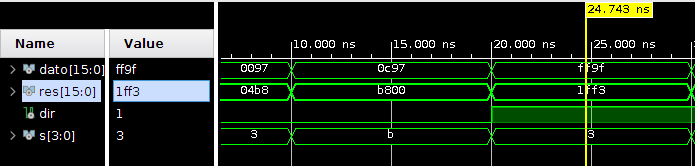
\includegraphics[scale=0.5]{imgs/tresBarrel.png}\\
  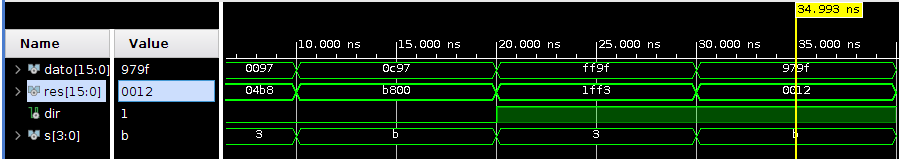
\includegraphics[scale=0.5]{imgs/cuatroBarrel.png}\\
\end{center}
\clearpage
\section{Diagramas RTL}
\subsection{Registro}
\begin{center}
  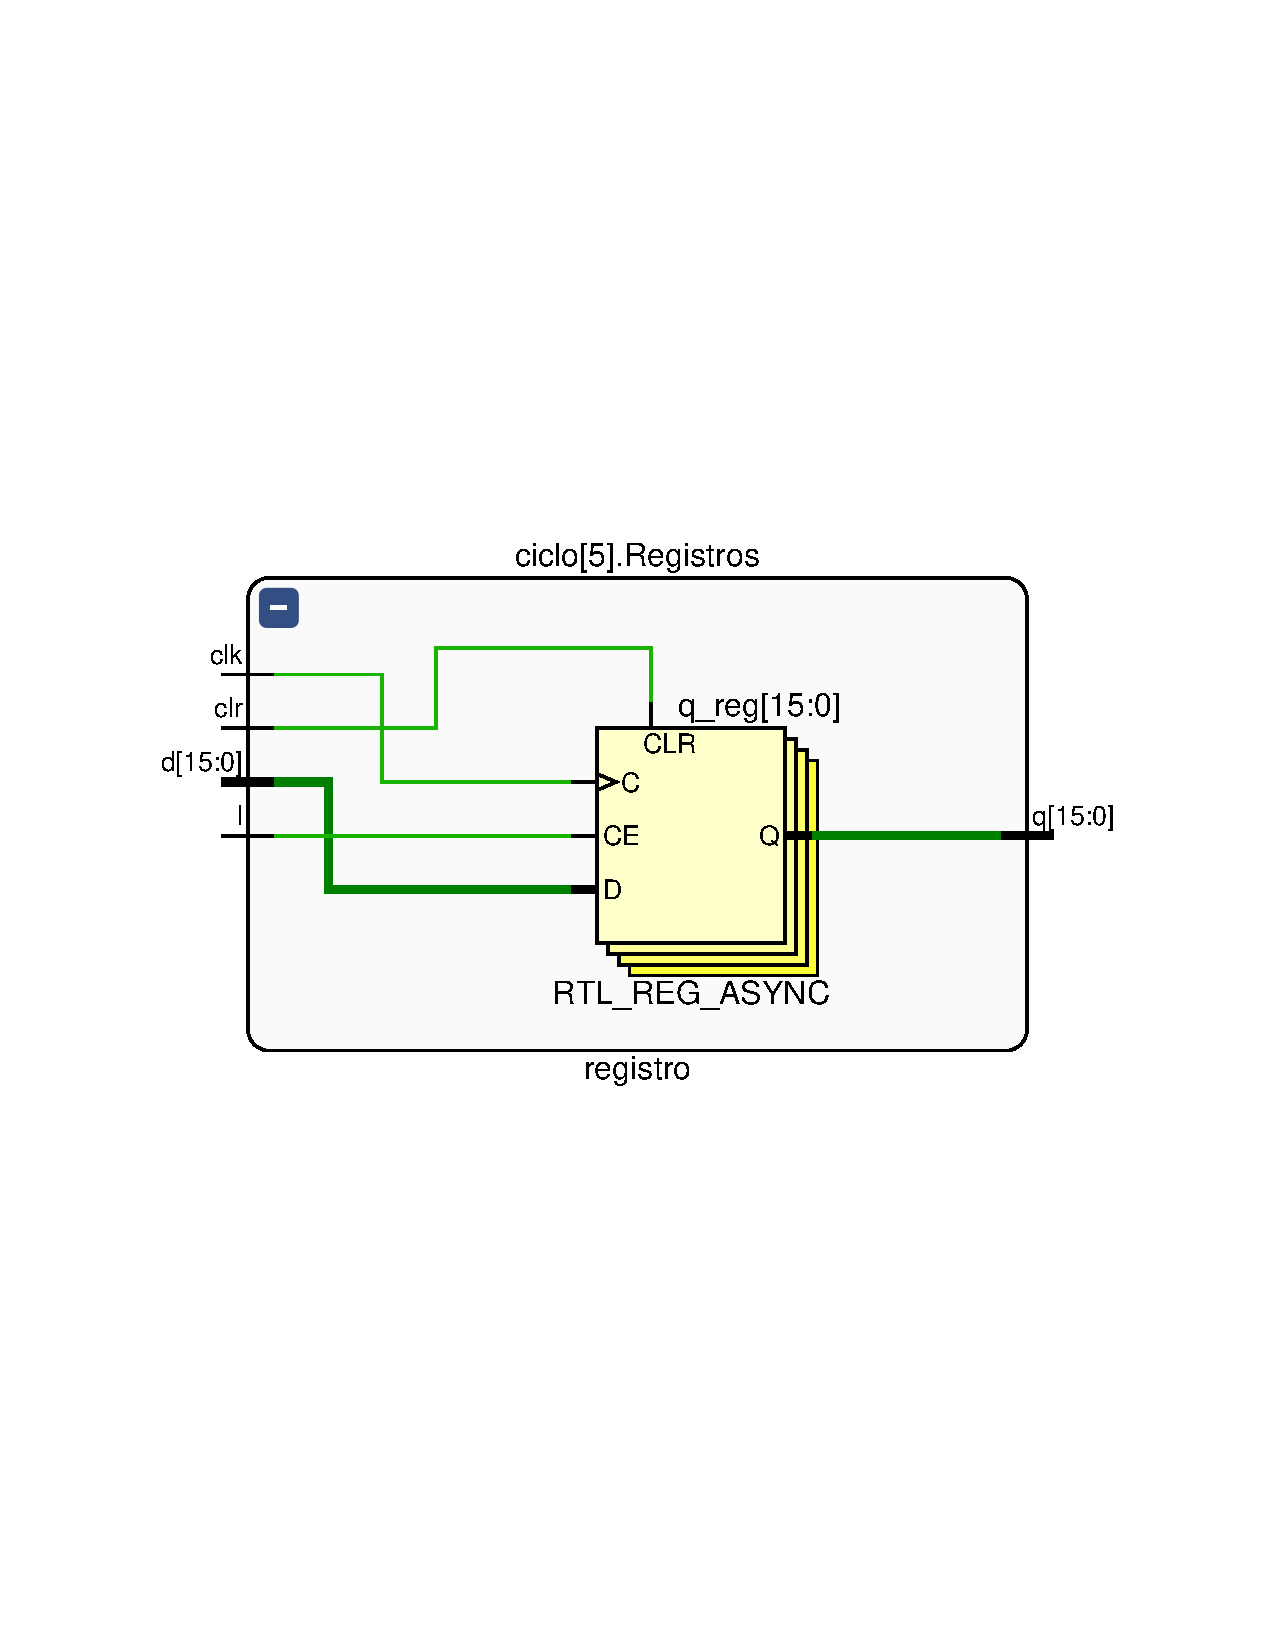
\includegraphics[scale=0.5]{sources/schematicRegistro.pdf}
\end{center}
\subsection{Mux 16 canales}
\begin{center}
  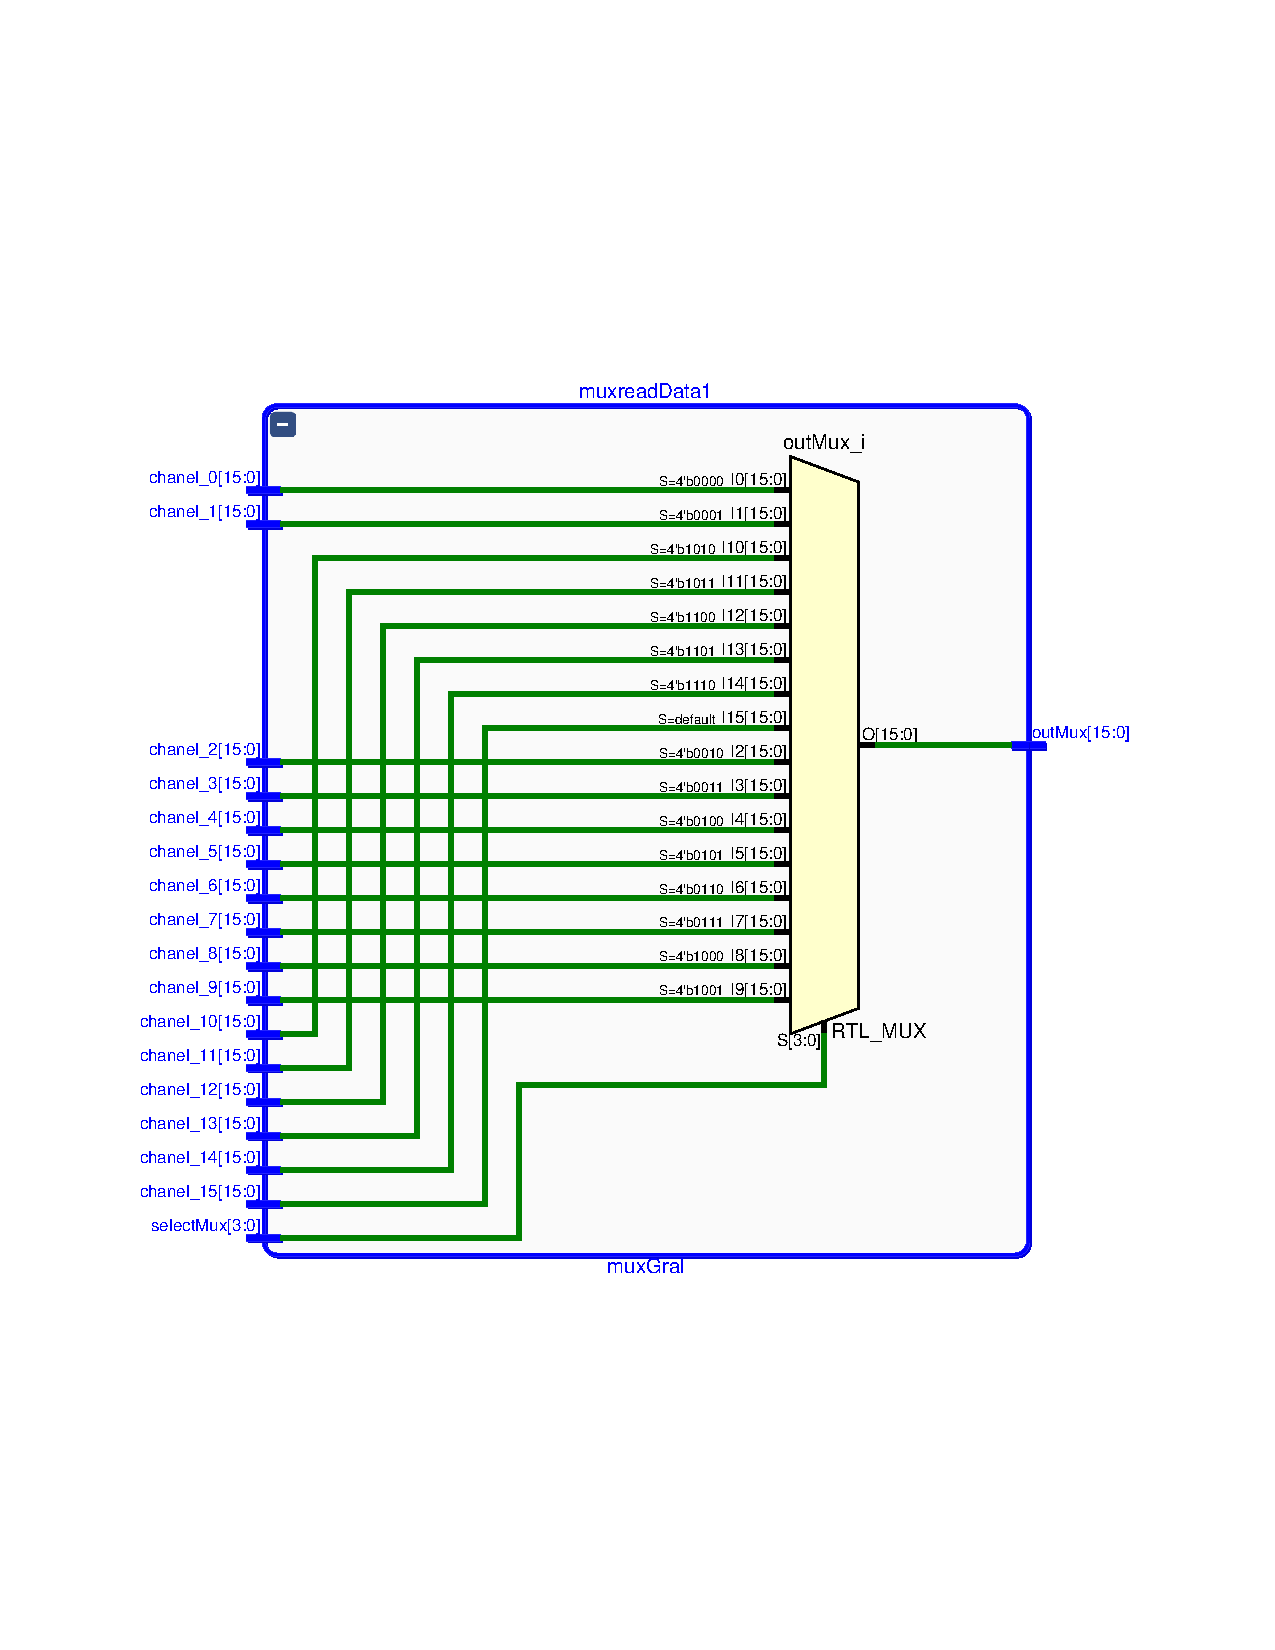
\includegraphics[scale=0.5]{sources/schematicMux16.pdf}
\end{center}
\subsection{Mux 2 canales}
\begin{center}
  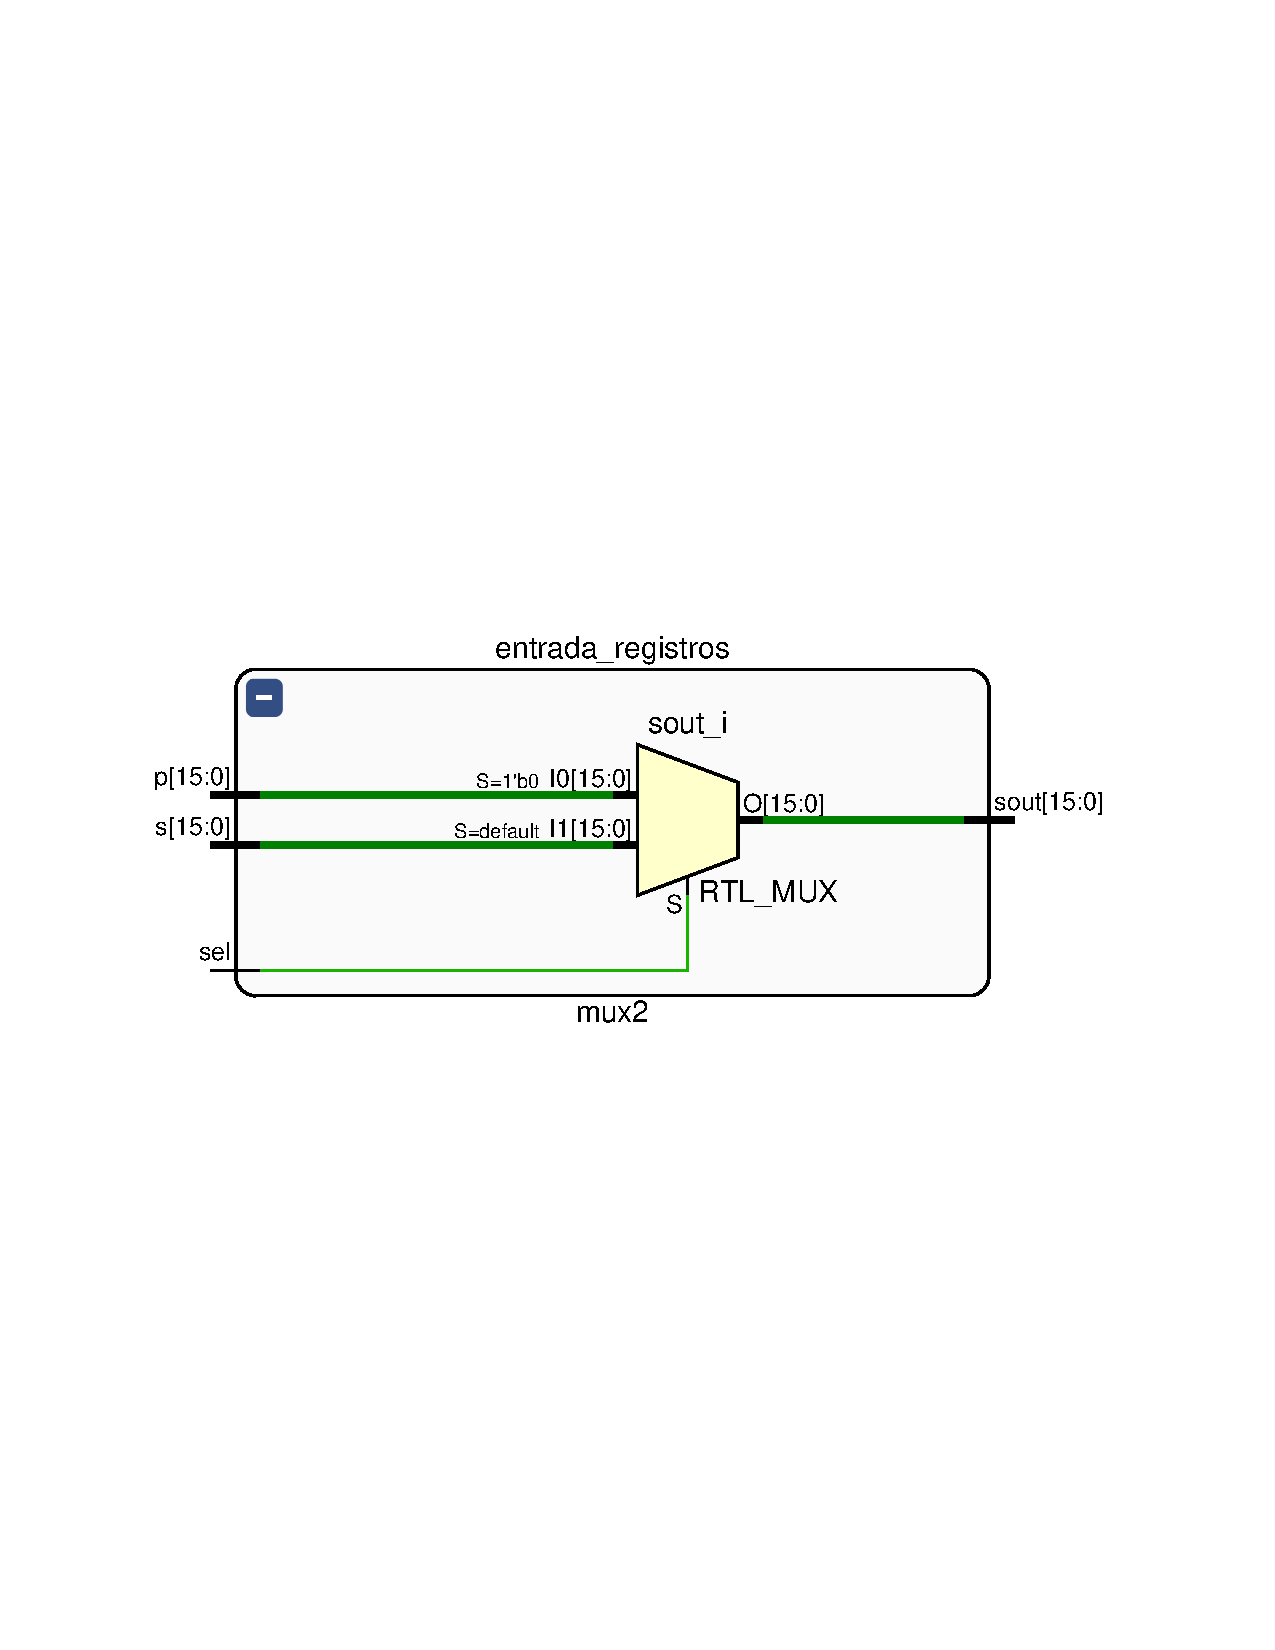
\includegraphics[scale=0.5]{sources/schematicMux2.pdf}
\end{center}
\subsection{Demux}
\begin{center}
  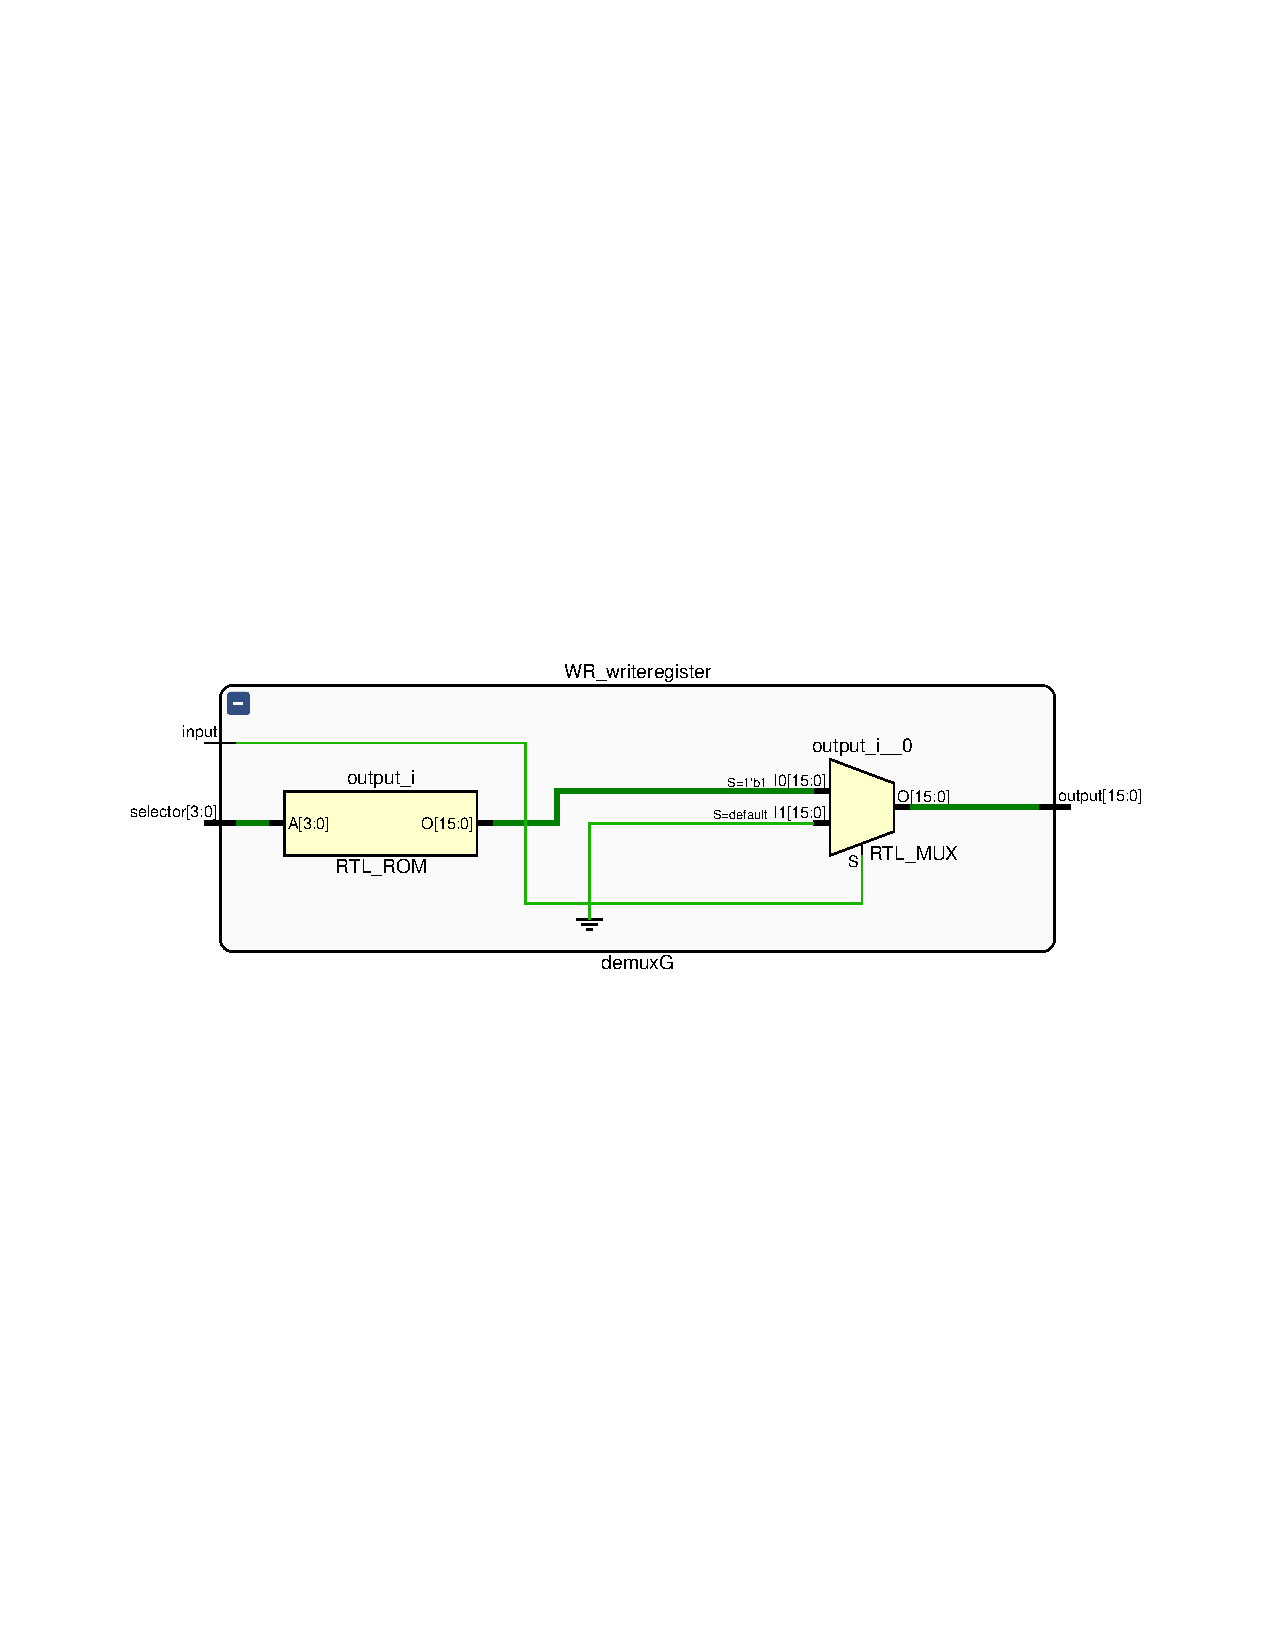
\includegraphics[scale=0.5]{sources/schematicDemuxRTL.pdf}
\end{center}
\subsection{Barrel-Shifter}
\begin{center}
  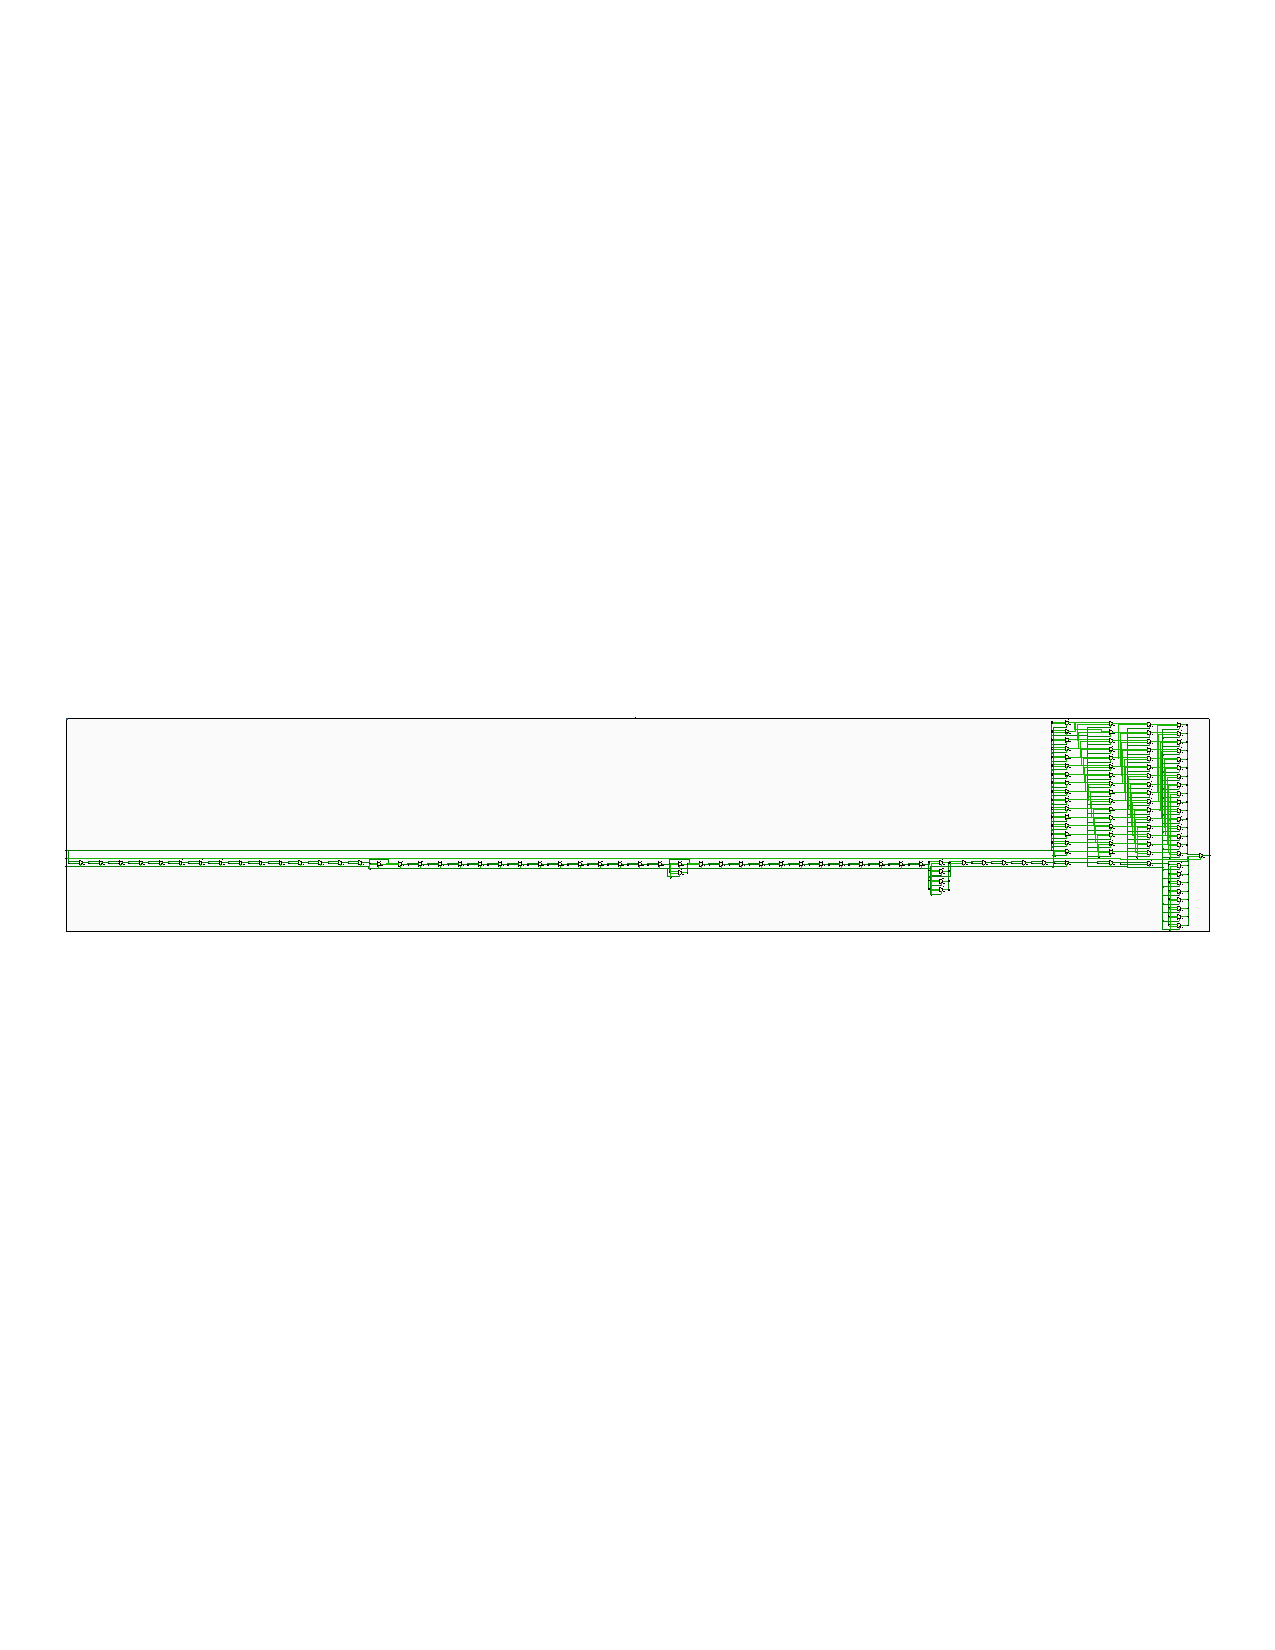
\includegraphics[scale=0.5]{sources/schematicBarrel.pdf}
\end{center}
\subsection{Archivo de Registros}
\begin{center}
  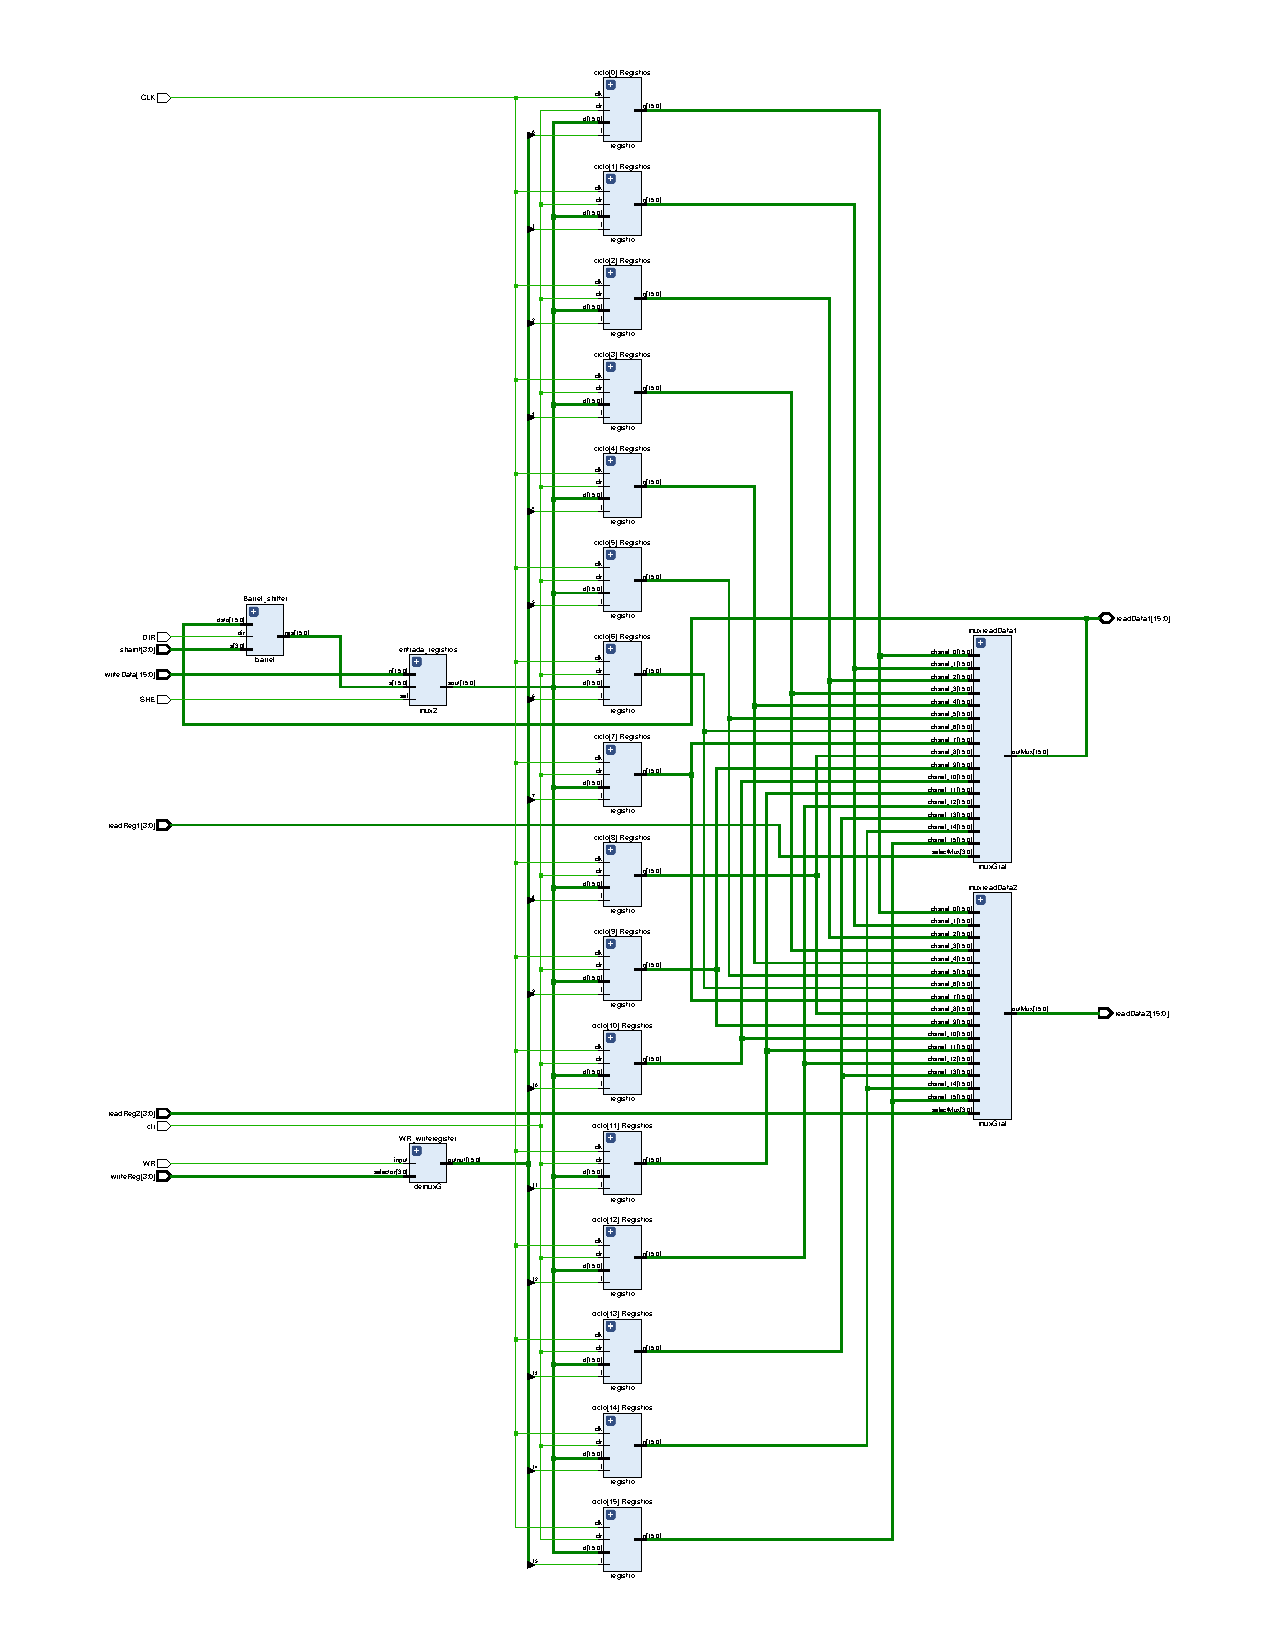
\includegraphics[scale=0.5]{sources/schematicArchReg.pdf}
\end{center}

\end{document}
